%% using aastex version 6


\newcommand{\opsfp}{N$_{FP_{obs}}$}
\newcommand{\opspc}{N$_{PC_{obs}}$}
\newcommand{\opsN}{N$_{obs}$}
\newcommand{\trueopspc}{T$_{PC_{obs}}$}
\newcommand{\missedfp}{T$_{FP_{obs}}$ - N$_{FP_{obs}}$}
\newcommand{\invfp}{N$_{FP_{inv}}$}
\newcommand{\invpc}{N$_{PC_{inv}}$}
\newcommand{\invN}{N$_{inv}$}
\newcommand{\sfatce}{SFA-TCE}


We use the \injtce\, \scrtce\ and \invtce\ data sets to determine the performance of the Robovetter, \S\ref{s:robovetter}, and measure its completeness and reliability.

\subsection{Completeness}
Completeness is the fraction of true transits that we detect and is calculated by dividing the number of on-target \injtce s (N$_{inj}$) by the number that are turned into PCs (N$_{PC_{inj}}$). 

\begin{equation}
\label{comp}
C = \frac{N_{PC_{inj}}}{N_{inj}}
\end{equation}



\subsection{Reliability}
\label{s:relcalc}
To assess the catalog reliability, we will assume that the \scrtce s and \invtce s are similar to those we see in the \opstce\ set. Close visual inspection of many in the sample validates that assumption.  One way to calculate the reliability of the catalog from our false alarm sets is to first calculate our effectiveness at correctly identifying a known false alarm as such.  Then given the number of false alarms we identify in the \opstce\ set, we can determine the reliability of the catalog against the type of false alarms present in the the simulated sets (\invtce\ and \scrtce). This method assumes the frequency of the different types of false alarms is well emulated by the simulated data sets. 


Effectiveness ($E$) is defined as the fraction of false positives correctly identified as false positives in the \opstce\ data set. 
\begin{equation}
\label{effect1}
E \equiv \frac{N_{FP_{obs}}}{T_{FP_{obs}}}
\end{equation}
Notice we are using N to indicate a measurable number, and T to indicate the ``True" number, assuming $E\leq 1 $.  If the simulated false alarm TCEs (for our derivation here we use \invtce\ to represent the set of simulated false alarms) accurately reflects the \opstce\ false positives, $E$ can be calculated as the number of simulated false alarm TCEs identified as false positives (\invfp) divided by the number of inverted TCEs (\invN). 

\begin{equation}
\label{effect2}
E = \frac{N_{FP_{inv}}}{N_{inv}}
\end{equation}

Reliability, $R$, is defined as the ratio of the true observed PCs (\trueopspc) to the total number of observed PCs (\opspc). At this point we can drop the \textit{obs} and \textit{inv} designation as all the inversion values are wrapped up in $E$, and the $N$ values shown below refer entirely to the number of candidates (PC) or false positives (FP) determined to be the \opstce set so that $N=N_{PC} + N_{FP}$. From the definition for reliability, we rewrite in terms of the number of true false positives.

\begin{equation}
R \equiv \frac{T_{PC}}{N_{PC}} =  1 + \frac{T_{PC}-N_{PC}}{N_{PC}} 
= 1 + \frac{N_{ops} - T_{FP} - N_{PC}}{N_{PC}}
\end{equation}

Substitute $N_{FP}=N-N_{PC}$ and you get another useful way to think about reliability, as the number of unidentified false positives relative to the number of candidates.

\begin{equation}
\label{rel}
R = 1 - \frac{T_{FP}-N_{FP}}{N_{PC}}
\end{equation}

However, the true number of observed FPs is not known. Using the effectiveness value measured from inversion (or scrambling) (equation \ref{effect2}) and combining it with our definition for effectiveness (equation \ref{effect2}), we get (T$_{FP}$):
\begin{equation}
T_{FP} = \frac{N_{FP}}{E} 
\end{equation}

Substituting into equation \ref{rel},
\textbf{
\begin{equation}
R= 1 - \frac{N_{FP}}{N_{PC}}(\frac{1-E}{E})
\end{equation}
}.

%or, in terms of the unreliability ($U= 1-R$) and the Ineffectiveness ($I=1-E$)
%\begin{equation}
%U=\frac{N_{FP}}{N_{PC}}(\frac{I}{E})
%\end{equation}

%\subsubsection{Example}

%If you choose one MES/Period bin, you can use the inversion effectiveness to calculate the reliability of the catalog for this bin. We show one example of the robovetter run below. If we consider the MES range of 10-20 and the Period range of 10-200 days, we find that the robovetter has $E=97.7\%$. The number of false positives in that bin is 2613 and the number of PCs is 730.  Thus the reliability is $1 - \frac{2613}{730} \times \frac{1-.977}{.977} = 91.7\% $.  This means that of the 730 reported PCs, 60 are actually false positives.

If the number of observed false positives is much larger than the number of false positives identified in the inversion run, it is possible to get a negative reliability. This likely means that we do not have a good measure of the effectiveness.  Given the number of observed false positives, we should have found more planet candidates than we did. Or, given the measure of the effectiveness, the number of FPs that were missed is greater than the number of PCs that we have left to draw from.  This can happen if the effectiveness measured by inversion is lower than the true value. For example, if the number of hard-to-identify false alarms is larger in the \invtce\ data set than in the \opstce\ data set.   

%-----------------------
%-----------------------
\subsection{The Similarity of the Simulated False Alarms}
\label{s:simularity}
In order to use the \scrtce\ and \invtce\ sets to determine the reliability of our catalog we must assume that the properties of these simulated false positives are similar to those of the false positives in the \opstce\ set.  Specifically, this simulated data should emulate the observed not-transit-like false positives.  There are many different reasons a false positive will fit in this category, e.g. instrumental noise and stellar spots. The method we use to measure reliability, outlined above, hinges on the assumption that for a certain parameter space the fraction of FP TCEs of a particular type is the same between the simulated and observed data sets.  This is the primary reason that we removed the TCEs caused by KOIs and EBs in the simulated data sets, see \S\ref{s:clean}. Inverted EBs and transits are not the type of false positive in the \opstce\ data set.  Since the Robovetter is very good at eliminating inverted transits, if they were included, we would have an inflated value for the effectiveness, and thus an inflated reliability. 

Figure\,\ref{f:tces} demonstrates that the number of TCEs from inversion and scrambling individually is smaller than the number of false positives in the \opstce\ set. This is in part due to the fact that by removing the stars that contain EBs and KOIs, we searched a significantly smaller number of stars for instances of false positives. The deficit is also caused by the fact that all types of false positives are not accounted for in these simulations. For instance, the \invtce\ set will not reproduce false positives caused by sudden dropouts in pixel sensitivity caused by cosmic rays. The \scrtce\ set will not reproduce the image artifacts from rolling band because the artifacts are not as likely to line-up at exactly one \Kepler -year.  However despite these problems, the relative number of false positives in these simulated data sets resembles that of the \opstce\ false positive population, especially if the two sets are combined.

Another way to judge how well the simulated data set matches the type of false positives in the \opstce s is by look at some of the Robovetter metrics.  Each metric measures some aspect of the TCE. For example, the LPP-metric measures whether the folded and binned light curve is transit shaped, and Skye measures whether the individual transits are likely due to rolling band.  If the simulated TCEs can be used to measure reliability in the way described above, then the the fraction of false alarms in any period bin caused by any particular metric should match between the two sets.  In Figure~\ref{f:fractionFailMetric} we show that this is basically true for both \invtce s and \scrtce s, especially for periods longer than 100 days and MES less than 15.  Keep in mind that more than one metric can fail any particular TCE, so the sum of the fractions across all metrics will be greater than one.  The deviations between TCE sets can be as large as 40 per cent for certain period ranges and such difference may cause systematic errors in our measurements of reliability.  But, since the types of false positives overlap, it is not clear how to propagate this information into a formal systematic error bar in the reliability.  

For our discussion of the reliability estimate, we are satisfied with this basic agreement. Given that neither of the two sets perform better across all regions of parameter space, and since more simulated false positives improves the precision on effectiveness,  we have decided to calculate the catalog reliability using a union of the \scrtce\ and \invtce\ set after they have been cleaned as described in \S\ref{s:clean}.  


%Both \scrtce\ and \invtce\ sets, their Robovetter dispositions and metrics are available at the NASA Exoplanet Archive.
%users may chose to redo this analysis with a different set of simulated false alarms to improve upon our estimates or to get a handle on accurate error bars.   

\begin{figure*}[h!]
    \centering
    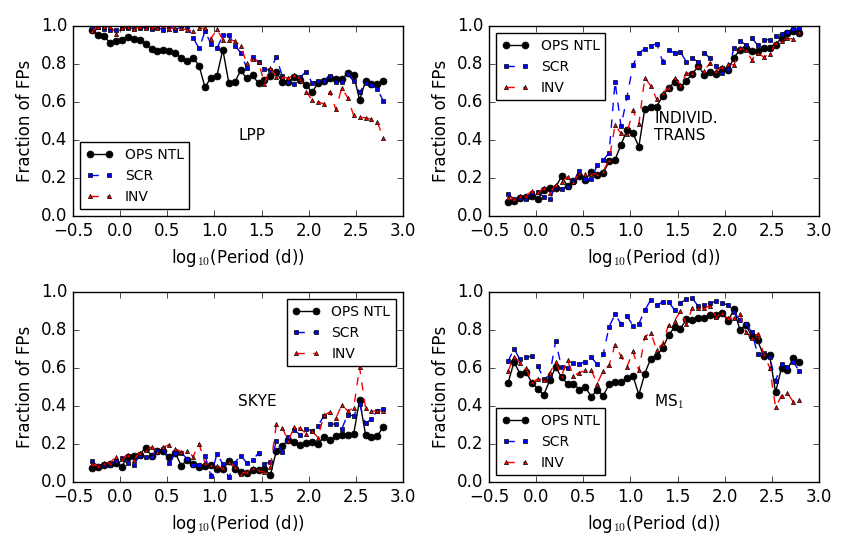
\includegraphics[width=0.9\linewidth]{fig-fractionFailsByMetric.png}
    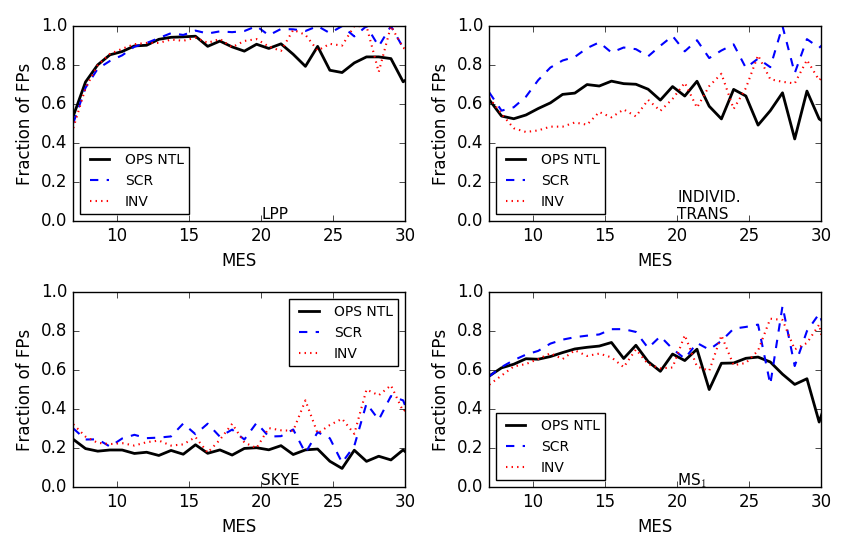
\includegraphics[width=0.9\linewidth]{fig-fractionFailsByMetricMes.png}
    \caption{The fraction of false positives failed by a particular type of Robovetter metric plotted against the logarithm of the period (top) or linear MES (bottom).  The fraction is plotted for not-transit-like FPs from the \opstce\ set in black, the \scrtce\ set in blue and the \invtce\ set in red. For each metric we include fails from either detrender (DV or Alt) for the metric stated in the middle of the plot. Upper left: LPP metric failures. Upper Right: TCEs that fails after removing a single transit due to any of the individual transit metrics.  Lower left: TCEs that fail after removing a single transit due to the Skye metric. Lower right: Model Shift 1 metric failures. }
    \label{f:fractionFailMetric}
\end{figure*}

%\begin{figure*}
%    \centering
    
%    \caption{The fraction of false positives failed by a particular type of Robovetter metric plotted against MES.  The fraction is plotted for not-transit-like FPs from the \opstce\ set in black, the \scrtce\ set in blue and the \invtce\ set in red. For each metric we include fails from either detrender (DV or Alt) for the metric stated in the middle of the plot. Upper left: LPP metric failures. Upper Right: TCEs that fails after removing a single transit due to any of the individual transit metrics.  Lower left: TCEs that fail after removing a single transit due to the Skye metric. Lower right: Model Shift 1 metric failures. }
%    \label{f:fractionFailMetricMes}
%\end{figure*}